\documentclass{article}
\linespread{1.5}
\usepackage[letterpaper, margin=1in]{geometry}
\usepackage{graphicx}
\usepackage{amsmath}
\begin{document}

\begin{center}
{\huge Homework 2}
\end{center}

\section{Image compression using clustering}
\bigskip

\subsection{detail}
I choose to implement the algorithm provided in The Elements of Statistical Learning (Hastie, Tibshirani, Friedman). For given cluster assignments C, the current estimate of cluster center is $m_k = x_i_k, \quad k = 1, 2, ..., K$. For each observation $x_i$, assign its cluster by minimizing total distance to cluster center, therefore their assignment is $i_k = argmin \sum_{C(i')=k} D(x_i, m_k)$. Then, update center $m_k$ by averaging all the data points in that cluster C, then the updated center $m_k'$ is chosen to be the closest point $x_i \in \mathcal C_k$ to the mean $\overline{xi} \in \mathcal C_k$. Iterate steps 1 and 2 until the assignments do not change.
\medskip

For K-medoids algorithm, because we store our data as pixels that contain RGB information, I decide to implement the city block (Manhattan) distance to compute distances between data points and clusters. In RGB color, each parameter (red, green, and blue) defines the intensity of the color as an integer between 0 and 255. Thus one pixel takes all of the three colors to represent its own color. So Manhattan distance which calculates,
$$
D(m_k, x_i) = \sum_{i = 1}^{N} |m_k - x_i| \quad m, x \in \mathcal{R}^N
$$
will summarize the overall ``intensity'' to travel from one color to another. Therefore, in our clustering assignment, we need to cluster most similar pixels into one group by minimizing these intensities.
\medskip

To minimize the computation expenses and accelerate running time, I set the maximum iteration to be 50 to prevent the program from timing out. (Based on the average iterations I observed from executing k-means algorithm).
\bigskip

\subsection{picture}
\medskip

\begin{center}
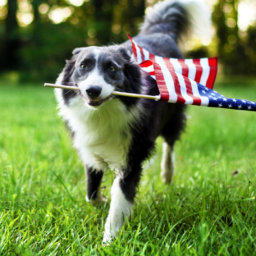
\includegraphics[scale=0.5]{dog}
\label{fig:dog original}
\end{center}

\subsection{Run your implementations with the picture you chose above, with several different K.}
\medskip

\begin{figure}[h!]
\centering
  \caption{Random Initialization, K=2}
  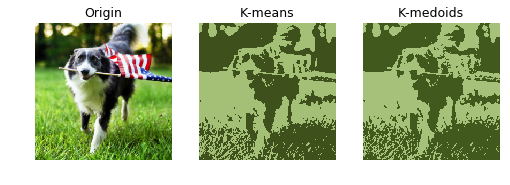
\includegraphics[scale=0.6]{dog_k2}
\end{figure}

By running both algorithms on the above picture and k = 2, I observed that k-means uses 16.58 seconds, and k-medoids uses 39.26 seconds. When k is small, the quality of the picture is compromised. They show only basic contours of the dog and the grass, but not details. When the cluster number is small, both the algorithms produce fairly the same result. The output quality are the same, and both robust. And in terms of the running time, k-means is better.
\bigskip

\begin{figure}[h!]
\centering
  \caption{Random Initialization, K=16}
  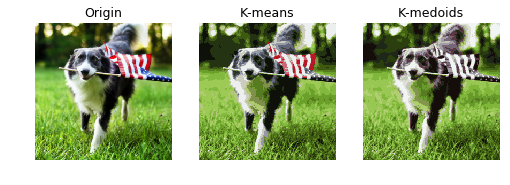
\includegraphics[scale=0.6]{dog_k16}
\end{figure}

By running both algorithms and set k equals to a larger value, 16, the output pictures are more similar to the original picture. They contain much more detail information of the original than they are when k is small. Yet I noticed significant differences between these two algorithms. When the cluster number increases, the running time differs tremendously. k-means uses 57.86 seconds (about 1 minute), and k-medoids uses 217.52 seconds (around 4 minutes). So for the k-means algorithm, it is still very quick to converge for large k. But for the k-medoids, it takes much more time to converge. 
\medskip

In terms of output quality, we can see that k-means algorithm produces result almost identical to the original picture. And it is much accurate and visually pleasant than the k-medoids' picture. K-medoid result seems to ``forget'' the red color by clustering it into gray. In terms of robustness, k-means is much more robust than k-medoids. 
\medskip

\begin{figure}[h!]
\centering
  \caption{Random Initialization, K=32}
  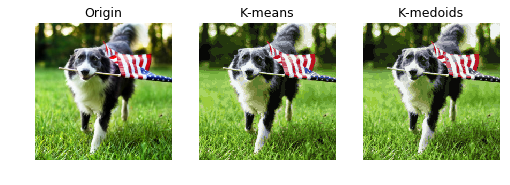
\includegraphics[scale=0.6]{dog_k32.png}
\end{figure}

When I increase k to be very large, 32, the output results for both algorithms are both identical to the original picture. That is great news - however, their running time differs even more than when k = 16. k-means uses 86.16 secons, while k-medoids uses 611.76 seconds (more than 10 minutes!). In terms of output quality, k-means still wins over k-medoids because the blue color is much better clustered in k-means. Thus, k-means is much more robust than k-medoids.

\subsection{Run your K-medoids implementation with different initial centroids/representatives}

\begin{figure}[h!]
\centering
  \caption{Poor Initialization, K=2}
  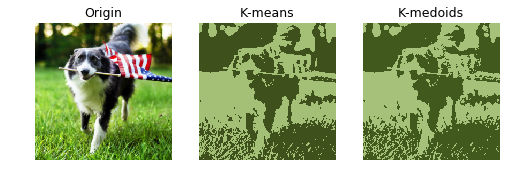
\includegraphics[scale=0.6]{dog_poor_2.png}
\end{figure}

In order to distinguish the differences, I intentionally assign poor centers. The poor assignments are chosen to be the very first 2 data points of the pixels (They are very likely to have the same color thus jeopardize the initialization). The results appear to be similar to the random assignments for both k-means and k-medoids algorithm. k-means uses 17.53 seconds, and k-medoids uses 16.90 seconds. The times do not have much variation neither. So in this case when k = 2, poor assignment does not affect the result for k-means but improves k-medois algorithm.
\medskip

\begin{figure}[h!]
\centering
  \caption{Poor Initialization, K=16}
  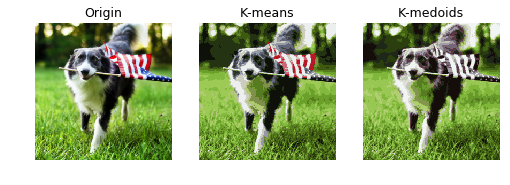
\includegraphics[scale=0.6]{dog_poor_16.png}
\end{figure}

\break
When increasing the cluster number to 16, and also initialize poor assignments to be the very first 16 data points, I observe similar result compared to random assignment. k-means uses 52.66 seconds (less than 1 minute), and k-medoids uses 202.80 seconds (about 4 minutes). The output quality are the same compared to random assignments. So in this case, poor assignments do not alter the result. 

\section{Spectral clustering}

\subsection{Proof}
Consider an undirected graph with non-negative edge weights $w_ij$ called adjacency matrix $W = \{w_ij'\}$. And G is a diagonal matrix with diagonal elements $g_i$ where $g_i = \sum_{i'} w_{ii'}$ is the sum of the weights of the edges connected to node i. Then, the graph Laplacian $L_{NxN} = G - W$.

For any vector $f = [f1, f2, ... f_N]$ we have
$$
f^TLf = \sum_{i=1}^N g_i {f_i}^2 - \sum_{i=1}^N \sum_{i'=1}^N f_i f_{i'} w_{ii'}
=\frac{1}{2} \sum_{i=1}^N \sum_{i'=1}^N w_{ii'} (f_i - f_{i'})^2
$$

The above equation suggests that a small value of $f^TLF$ will be achieved if pairs of points with large adjacencies have coordinates $f_i$ and $f_{i'}$ close together. Since $1^TL1 = 0$ for any graph, the constant vector $1 = [1, 1, .. ,1]$, which indicates that the graph is all connected - only one component, is the only eigenvector associated with eigenvalue zero.

Inspired from 1 component case, for a graph with m connected components, $A_1, A_2, ... A_m$, L can be reorganized as a block diagonal with a block for each connected component. For vector $f_1 = [1, 1, ..., 1, 0, ..., 0]$ which contain the indicator vector of component $I_{A_1}$, $f^TLf$ is minimized to zero. Thus, L has m eigenvectors of eigenvalue zero, and the eigenspace of eigenvalue zero is spanned by the indicator vectors of the connected components $I_{A_1}, ... , I_{Am}$. For example, for a graph that contain m perfectly connected components,
$$
\begin{bmatrix}
I_{A1}&0&0&0\\
0&I_{A2}&0&0\\
\vdots&\vdots&\ddots&\vdots\\
0&0&0&I_{A_m}\\
\end{bmatrix}
\begin{bmatrix}
\mathbf{1}\\
0\\
0\\
0\\
\end{bmatrix}
= 0 \times 
\begin{bmatrix}
\mathbf{1}\\
0\\
0\\
0\\
\end{bmatrix}
=
\begin{bmatrix}
0\\
0\\
0\\
0\\
\end{bmatrix}
$$
which the above eigenvector is a generalizetion of the true eigenvector. There are m such eigenvectors corresponding to eigenvalue zero, and the indicator vectors \textbf{1} of these components span the zero eigenspace. In other words, there are m eigenvectors associated with eigenvalue zero who best represent each component within graph Laplacian L.

\subsection{Real data: political blogs dataset}
The false classification rate is 51.54\%.

\section{PCA: Food consumption in European area}

We can easily see that Luxembourg has different dietary habit from other countries.

\begin{figure}[h!]
\centering
  \caption{projections}
  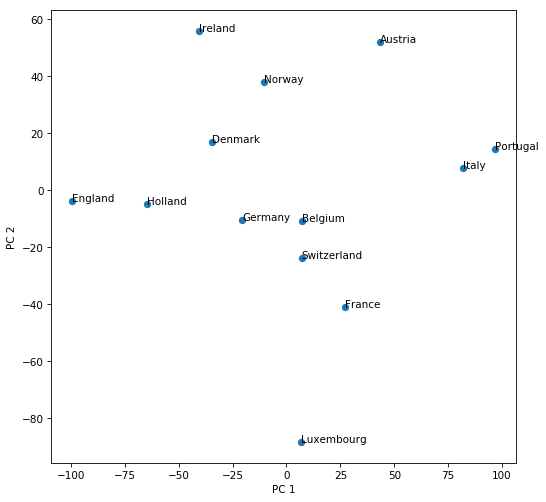
\includegraphics[scale=0.6]{Q3.png}
\end{figure}

\end{document}